\documentclass{beamer}
\usepackage{beamerthemesplit}
\usepackage{graphics}
\logo{
\includegraphics[height=1cm]{psi_logo_white.png}}
\usetheme{Pittsburgh}
\usecolortheme{dove}
\beamertemplatenavigationsymbolsempty
\setbeamertemplate{footline}[frame number]
\definecolor{myback}{RGB}{175,238,238}
\setbeamercolor{structure}{bg=myback}
\usepackage[T1]{fontenc}
\newcommand{\changefont}[3] {
 \fontfamily{#1} \fontseries{#2} \fontshape{#3} \selectfont}

\title{NeXus Code Camp}
\author{Mark K\"onnecke }
\institute{Paul Scherrer Institute\\Switzerland }
\date{\today} 

\begin{document}

\begin{frame}
\titlepage
\end{frame}

\begin{frame}
\frametitle{API Topics}
\begin{itemize}
\item NXclonehandle
\item PHDF-driver
\item PyTree-API
\item C++ Tree API
\item Cmake
\item NXdict replacement design based on NXDL
\item NXvalidate
\item HDF-5 1.8.*
\item Fedora installer
\item 64 bit dataset sizes
\item All dimensions unlimited
\end{itemize}
\end{frame}

\begin{frame}
\frametitle{General Topics}
\begin{itemize}
\item WWW-site from Manual
\item NeXus for the impatient
\item Encoding of axis dependencies
\item Handling multi dimensional scans
\item Sphinx discussion
\item Cleanup NeXus applications
\item NXdetetcor and Dectris
\end{itemize}
\end{frame}


\begin{frame}
\frametitle{Presentations}
\begin{itemize}
\item Cmake (Freddy)
\item Sphinx (Pete J.) 
\item PHDF (Mark)
\item HDF-5 1.6 to 1.8 (Freddy)
\item C++ Tree API (Eugen W.)
\item Public NeXus Talk (Mark K.) 
\end{itemize}
\end{frame}

\begin{frame}
\frametitle{Technical 1}
\begin{itemize}
\item NXclonehandle
\begin{itemize}
\item NAPI was made threadsafe on the last code camp
\item Each thread needs a file handle: NXclonehandle
\end{itemize}
\item PHDF: driver for parallel HDF-5 to write and read really fast
\item PyTree API:
\begin{itemize}
\item Writen by Ray Osborn
\item Still needs unit tests
\item Critical for 4.3 NAPI release
\end{itemize}
\end{itemize}
\end{frame}

\begin{frame}
\frametitle{Technical 2}
\begin{itemize}
\item Eugen Wintersberger presents us his C++ tree API
\item NXdict replacement:
\begin{itemize}
\item NXdict is an additional C-API 
\item Describes path of item in NeXus file via an external file
\item NXdict calls create structure as needed 
\item CHANGE: use NXDL 4 structure description
\item CHANGE: review API
\item Inspiration: CDM-API
\item Seek collaboration with CDM? Affects also C++ API
\end{itemize}
\end{itemize}
\end{frame}

\begin{frame}
\frametitle{Technical 3}
\begin{itemize}
\item Switch from autoconf to Cmake
\item NXvalidate: needs completion
\item HDF-5 1.6.* to 1.8.*
\item Fedora (rpm) installer
\item 64 bit sizes: Freddie has to many events
\item NX\_UNLIMITED all over, HDF-5: yes, HDF-4, XML: No
\end{itemize}
\end{frame}

\begin{frame}
\frametitle{NeXus for the Impatient}
\begin{itemize}
\item Short Manual (8 pages) about what NeXus is all about
\item Content
\begin{itemize}
\item Key Concepts
\item NeXus Benefits
\item Where do I find information?
\item How to access my data?
\item NeXus examples
\item Use cases
\end{itemize}
\end{itemize}
\end{frame}


\begin{frame} \frametitle{Axis Dependency Encoding}
\begin{itemize}
\item Decided: extend NeXus to allow full mapping from CBF to NeXus
\item Information to encode:
\begin{description}
\item[type] rotation or translation: DONE! transformation\_type attribute
\item[direction] vector around which to rotate or along which to translate: DONE! attribute
\item[value] The angle of rotation or the length of translation, DONE!
\item[dependency] The order of operations to place a component, to be discussed!
\end{description}
\end{itemize}
\end{frame}


\begin{frame} \frametitle{Expressing Axis Dependency in NeXus}
\begin{itemize}
\item Implied: use existing NeXus coordinate system
\item dependson attribute pointing to depending axis
\item transform field in base classes which becomes a comma separated list of 
 the path to the transformations required to position this component
\item Create a special container to hold axis dependencies, NXdependency, to 
 collect the dependencies in one place for easy access. This is what CIF does
\end{itemize}
\end{frame}

\begin{frame} \frametitle{Dependons Option}
\begin{tabbing}
\hspace*{1cm} \= \hspace*{1cm} \= \hspace*{1cm} \= \hspace*{1cm} \= \hspace*{1cm} \= \hspace*{1cm}\= \kill
\>sample,NXsample\\
\> \>rotation\_angle\\
\> \>chi (dependson rotation\_angle)\\
\> \>phi (dependson phi)\\
\end{tabbing}
\end{frame}

\begin{frame} \frametitle{Transform Option}
\begin{tabbing}
\hspace*{1cm} \= \hspace*{1cm} \= \hspace*{1cm} \= \hspace*{1cm} \= \hspace*{1cm} \= \hspace*{1cm}\= \kill
\>sample,NXsample\\
\> \>rotation\_angle\\
\> \>chi \\
\> \>phi \\
\> \>transform = rotation\_angle,chi,phi \\
\end{tabbing}
\end{frame}


\begin{frame} \frametitle{Separate Group Option}
\begin{tabbing}
\hspace*{1cm} \= \hspace*{1cm} \= \hspace*{1cm} \= \hspace*{1cm} \= \hspace*{1cm} \= \hspace*{1cm}\= \kill
\>sample,NXsample\\
\> \>rotation\_angle\\
\> \>chi \\
\> \>phi \\
\>dependency,NXdependency\\
\> \>sample/chi = \\
\> \> \>sample/rotation\_angle\\
\> \>sample/phi =\\
\> \> \> sample/chi\\
\> \>instrument/detector/x\_translation = \\
\> \> \>instrument/detector/distance\\
\> \>instrument/detector/distance = \\
\> \> \>instrument/detector/polar\_angle\\
\end{tabbing}
\end{frame}



\begin{frame} \frametitle{Handling Multi-Dimensional Scans}
\begin{itemize}
\item Conflicting use cases:
\begin{itemize}
\item Easy plotting
\item Careful data analysis
\end{itemize}
\end{itemize}
\end{frame}

\begin{frame} \frametitle{Easy Plotting}
\begin{tabbing}
\hspace*{1cm} \= \hspace*{1cm} \= \hspace*{1cm} \= \hspace*{1cm} \= \hspace*{1cm} \= \hspace*{1cm}\= \kill
\>data,NXdata\\
\> \>data[nx,ny]\\
\> \> \>@signal=1 \\
\> \>x[nx]\\
\> \> \>@axis=1\\
\> \>y[ny]\\
\> \> \>@axis=2\\
\end{tabbing}
\end{frame}


\begin{frame} \frametitle{Careful Data Analysis}
\begin{tabbing}
\hspace*{1cm} \= \hspace*{1cm} \= \hspace*{1cm} \= \hspace*{1cm} \= \hspace*{1cm} \= \hspace*{1cm}\= \kill
\>data,NXdata\\
\> \>data[nx,ny]\\
\> \> \>@signal=1 \\
\> \>x[nx,ny]\\
\> \>y[nx,ny]\\
\end{tabbing}
\end{frame}

\begin{frame} \frametitle{Tobias Suggestion}
\begin{tabbing}
\hspace*{1cm} \= \hspace*{1cm} \= \hspace*{1cm} \= \hspace*{1cm} \= \hspace*{1cm} \= \hspace*{1cm}\= \kill
\>data,NXdata\\
\> \>data[nx,ny]\\
\> \> \>@signal=1 \\
\> \>x[nx,ny]\\
\> \> \>@axis=1,2\\
\> \> \>@label=1\\
\> \>y[nx,ny]\\
\> \> \>@axis=1,2\\
\> \> \>@label=2\\
\end{tabbing}
\end{frame}

\begin{frame} \frametitle{Marks Suggestion}
\begin{tabbing}
\hspace*{1cm} \= \hspace*{1cm} \= \hspace*{1cm} \= \hspace*{1cm} \= \hspace*{1cm} \= \hspace*{1cm}\= \kill
\>data,NXdata\\
\> \>data[nx,ny]\\
\> \> \>@signal=1 \\
\> \> \>@axes=x,y \\
\> \> \>@axesvalue=x\_scan,y\_scan \\
\> \>x[nx]\\
\> \> \>@axis=1\\
\> \>y[ny]\\
\> \> \>@axis=2\\
\> \>x\_scan[nx,ny]\\
\> \>y\_scan[nx,ny]\\
\end{tabbing}
\end{frame}

\begin{frame} \frametitle{More Suggestions?}
\begin{tabbing}
\hspace*{1cm} \= \hspace*{1cm} \= \hspace*{1cm} \= \hspace*{1cm} \= \hspace*{1cm} \= \hspace*{1cm}\= \kill
\>data,NXdata\\
\> \>data[nx,ny]\\
\> \> \>@signal=1 \\
\end{tabbing}
\end{frame}

\begin{frame}
\frametitle{NXdetector Extensions for Dectris}
\begin{itemize}
\item Dectris (Eiger, Pilatus, Mythen) going HDF-5 with NeXus conventions
\item Additions to NXdetector for this kind of detector
\item Programming model:
\begin{itemize}
\item Dectris writes HDF-5 file with NXdetector
\item Local DAQ-system adds beamline metadata   
\end{itemize}
\end{itemize}
\end{frame}




\begin{frame} \frametitle{Prioritise!}
\end{frame}














\begin{frame} \frametitle{Transformation Matrices}
\begin{math}
T = \left( \begin{array}{cccc}
1 & 0 & 0 & x\\
0 & 1 & 0 & y\\
0 & 0 & 1 & z\\
0 & 0 & 0 & 1\\
\end{array} \right)
\end{math}

\begin{math}
\onslide+<2-> 
R = \left( \begin{array}{cccc}
r11 & r12 & r13 & 0\\
r21 & r22 & r23 & 0\\
r31 & r32 & r33 & 0\\
0 & 0 & 0 & 1\\
\end{array} \right)
\end{math}

\end{frame}

\begin{frame} \frametitle{Combining Transformations}
\begin{figure}[!ht]
\resizebox{7cm}{5cm}{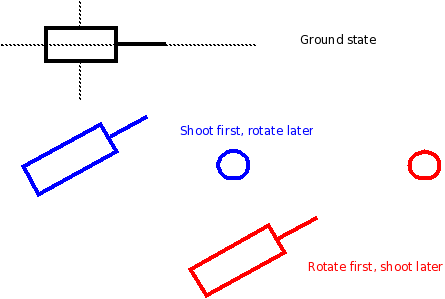
\includegraphics[width=0.75\textwidth]{rotcombi.png}}\end{figure}
\end{frame}

\begin{frame} \frametitle{Some Properties}
\begin{itemize}
\item Transformations can be combined by matrix multiplications
\item Individual matrices can be derived by looking at the situation when everything else is 0
\item Absolute positions can be obtained by multiplying the resulting matrix with its transpose
\item Defines new coordinate systems at components
\item CIF contains a duplication: vector, offset scheme 
\end{itemize}
\end{frame}

\begin{frame} \frametitle{What Use Is This?}
\begin{itemize}
\item Allows to calculate absolute positions of components in the laboratory coordinate systems
\item Can directly convert from a detector coordinate system to  
 vectors in Lab coordinate system
\item Calculate things like impact of primary beam on detector, SAS
\item Allows arbitray axis to be expressed
\item Intuitively describe an instrument with angles and translations and still be able
 to recover absolute coordinates
\end{itemize}
\end{frame}


\begin{frame} \frametitle{NeXus Axis Mapped}
\begin{itemize}
\item rotation\_angle, polar\_angle, rotate 0 1 0
\item azimuthal\_angle, rotate 0 0 1
\item distance, translate 0 0  1
\item chi, rotate 0 0 1
\item phi rotate, 0 1 0
\item NeXus polar coordinate system: rotate azimuthal\_angle, rotate polar\_angle, 
 translate by distance
\end{itemize}
\end{frame}

\begin{frame} \frametitle{CIF Dependency Table}
\begin{tabular}{llllll}
axis-id &type &equipment&dependson &vector & offset\\
gonio\_phi &rotation& goniometer & . &1,0,0,& ...\\
det\_z&translation&detector& .& 0,0,-1& 0 0 0\\
det\_y&translation&detector&det\_z&0,1,0&0,0,0\\
det\_x&translation&detector&det\_y&1,0,0&0,0,0\\
\end{tabular}
\end{frame}






\end{document}

\begin{frame} \frametitle{NeXus Simple Coordinate System }
\begin{figure}[!ht]
\resizebox{7cm}{5cm}{\includegraphics[width=0.75\textwidth]{polplane.png}}\end{figure}
\end{frame}

\begin{frame}
\frametitle{The Predicament of the Traveling Scientist}
\begin{itemize}
\item<1->A different data format wherever she goes
\item<2->Spends lots of time converting formats or writing readers
\item<3->Waits even longer to load data from inefficient data formats
\item<4->DA requires N files in different  formats, notes, local knowledge 
\item<5->Cannot read her collaborators data
\item<6->Has to keep extra information in yet another form
\end{itemize}
\end{frame}
